\documentclass{article}
\usepackage{graphicx} % Required for inserting images
\usepackage{amsmath}

\title{Lab 2 Report}
\author{Moaaz Mostafa Ibrahim \hspace{20pt} 2400862}
\date{}

\begin{document}
\maketitle
\section*{Question 1}
"a) Determine the value of R1 required to achieve an output voltage of Vo=5V when the binary input is $(1111)_2$.\\ 
\\
b) Verify your solution using MATLAB for the following binary inputs:\\
i. b3b2b1b0 = “0001”\\
ii. b3b2b1b0 = “1001”\\
iii. b3b2b1b0 = “1111”\\ 
\noindent
\textbf{Note}: Logic "1" corresponds to +5V, while logic "0" corresponds to 0V. "\\

\noindent
a) $V_{out} = 5 = R_f (V_{i1} + \frac{V_{i2}}{2} + \frac{V_{i3}}{4} + \frac{V_{i4}}{8}) = 5R_f (1 + \frac{1}{2} + \frac{1}{4} + \frac{1}{8})$\\

\noindent
$R_f = \frac{1}{1 + \frac{1}{2} + \frac{1}{4} + \frac{1}{8}} k\Omega \approx 533.333\Omega$\\

b)

\begin{figure}[h]
    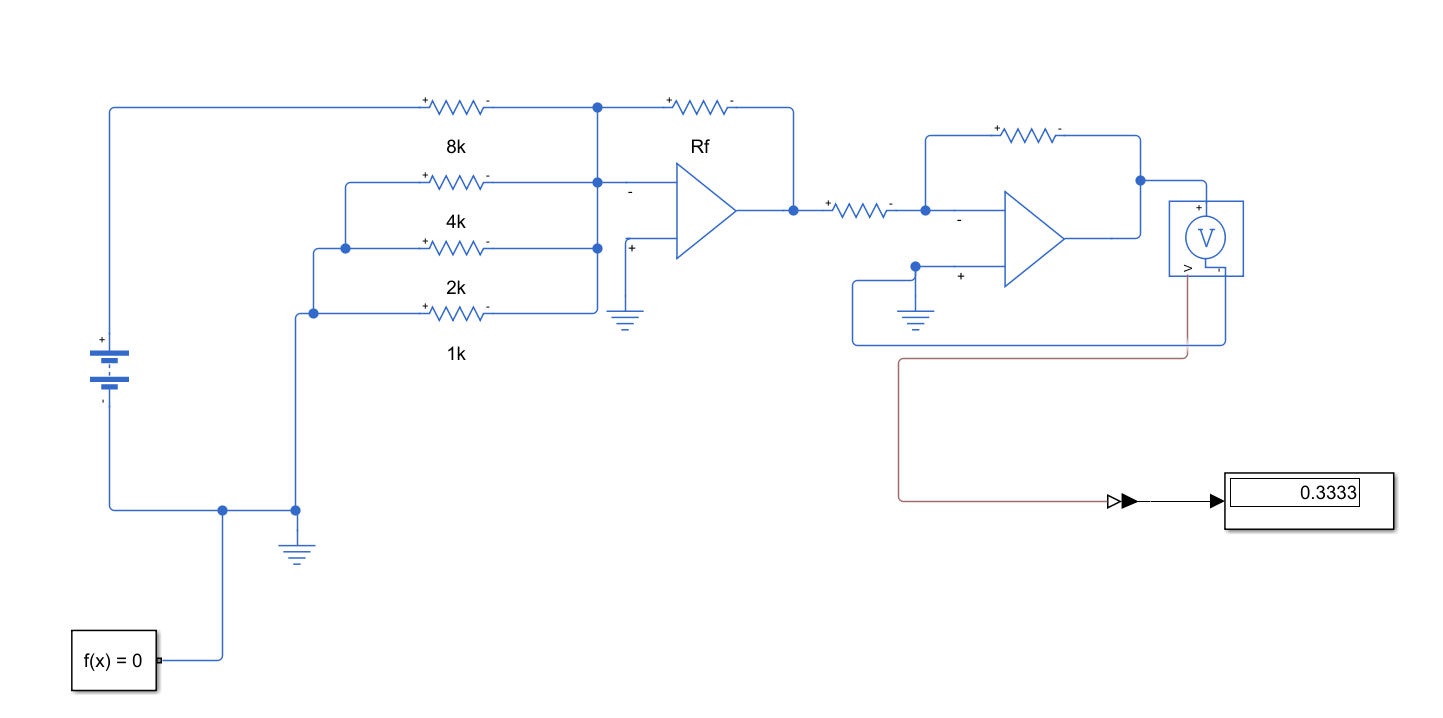
\includegraphics[width=0.75\linewidth]{Media/DAC-i.png}
\end{figure}

\begin{figure}[h]
    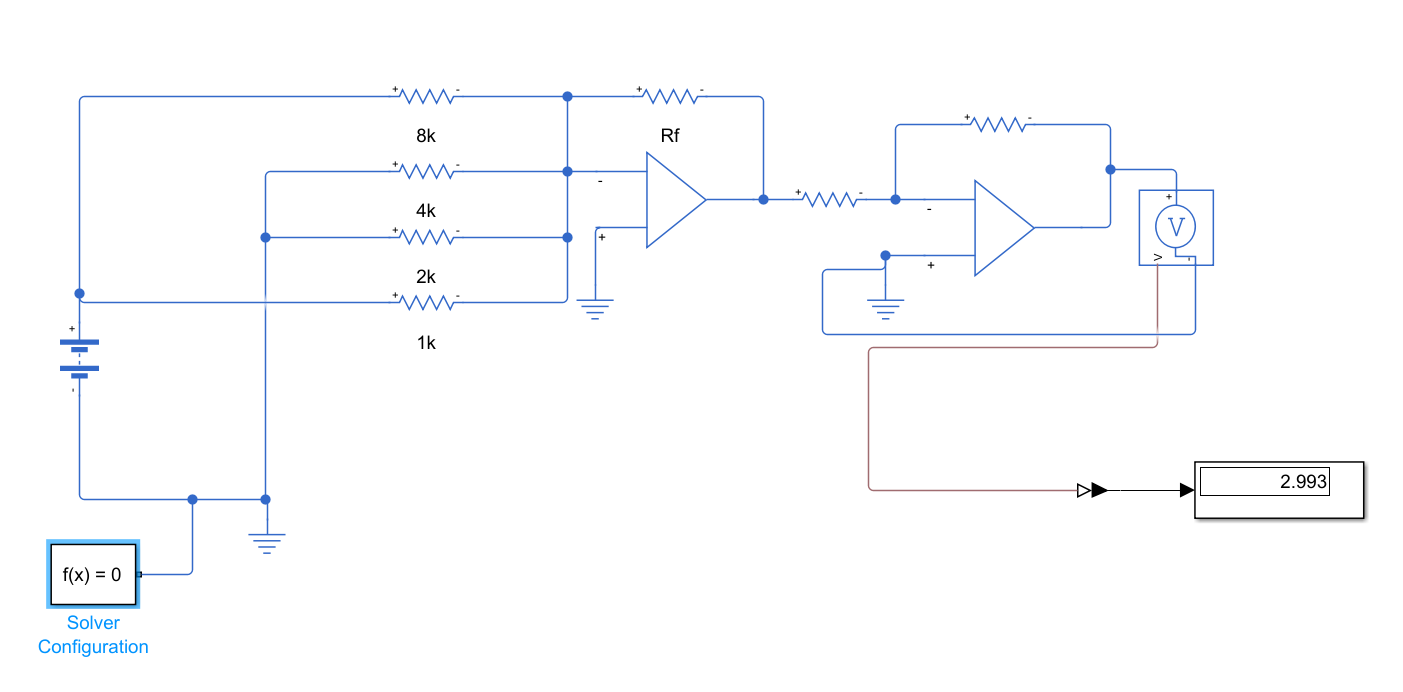
\includegraphics[width=0.75\linewidth]{Media/DAC-ii.png}
\end{figure}

\begin{figure}[h]
    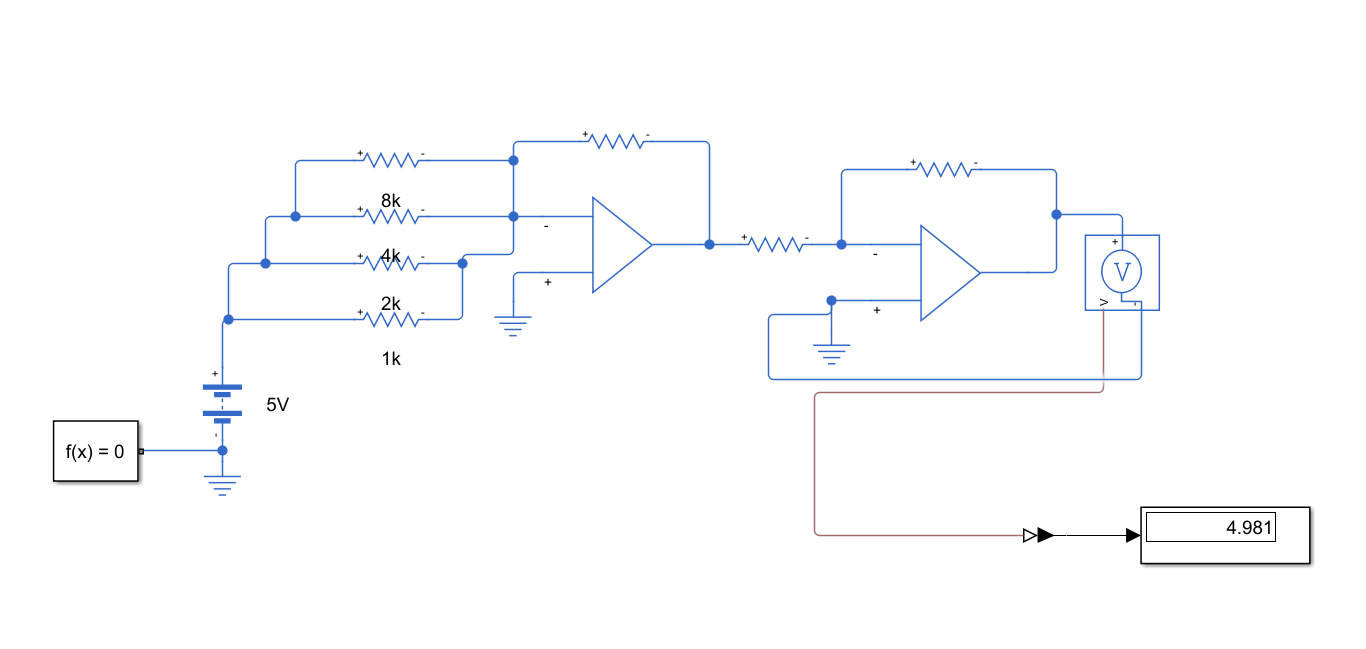
\includegraphics[width=0.75\linewidth]{Media/DAC-iii.png}
\end{figure}

\newpage
\section*{Question 2}
"Repeat Question 1 using the DAC circuit shown.\\
Hint: Calculate Vo using only two input values, then attempt to predict the remaining values based on the same pattern."\\

\noindent
a) $V_{out} = 5 = R_f (\frac{V_{b3}}{2} + \frac{V_{b2}}{4} + \frac{V_{b1}}{8} + \frac{V_{b0}}{16}) = 5R_f (\frac{1}{2} + \frac{1}{4} + \frac{1}{8} + \frac{1}{16})$\\

\noindent
$R_f = \frac{1}{\frac{1}{2} + \frac{1}{4} + \frac{1}{8} + \frac{1}{16}} k\Omega \approx 1066.66\Omega$\\

\newpage
\noindent
b)\\
\begin{figure}[h]
    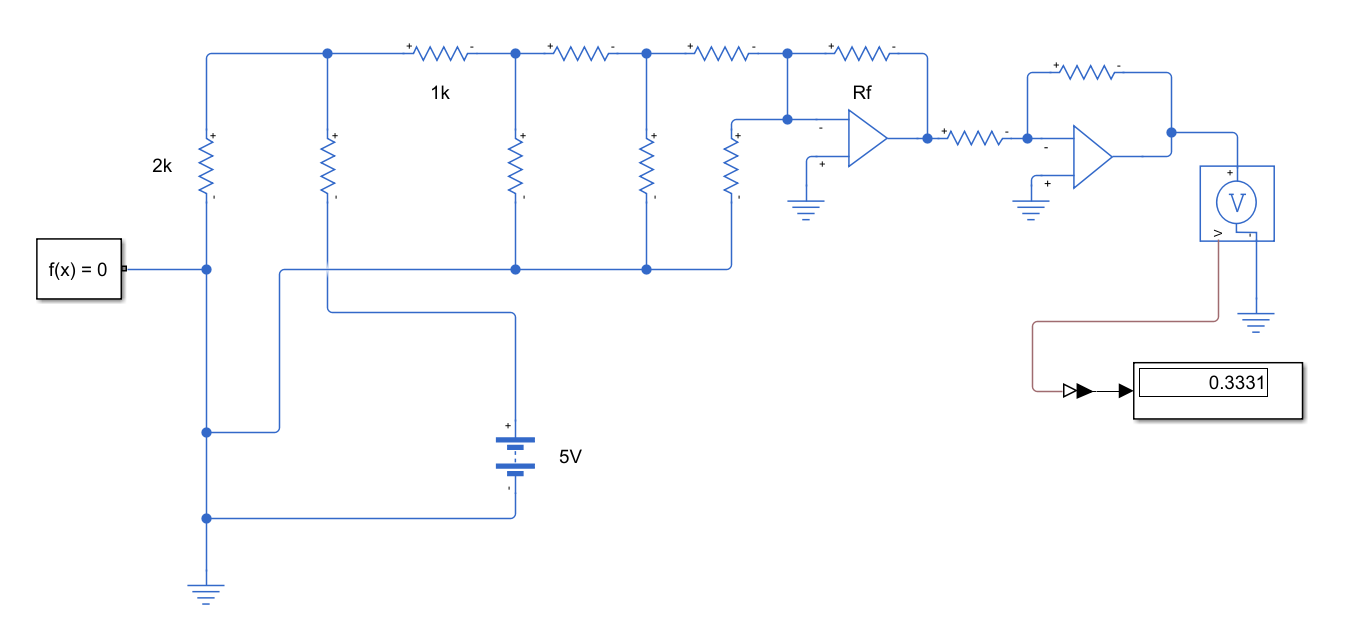
\includegraphics[width=0.75\linewidth]{Media/DAC2-i.png}
\end{figure}

\begin{figure}[h]
    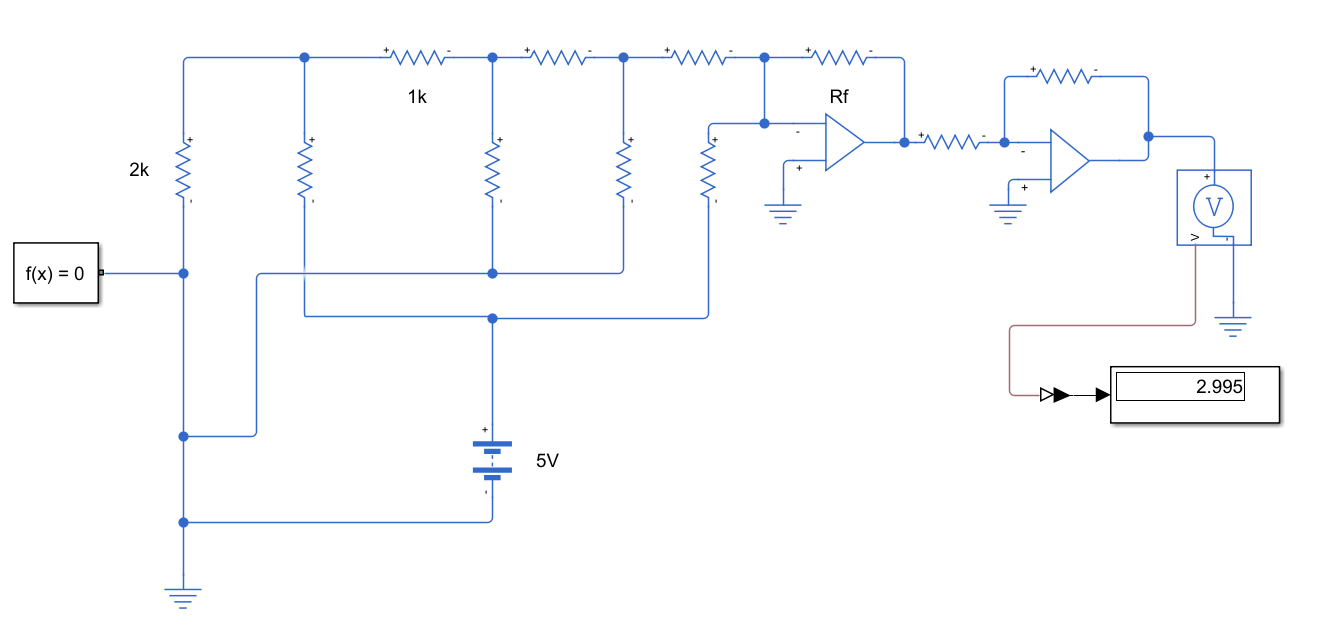
\includegraphics[width=0.75\linewidth]{Media/DACC2-ii.png}
\end{figure}

\begin{figure}[h]
    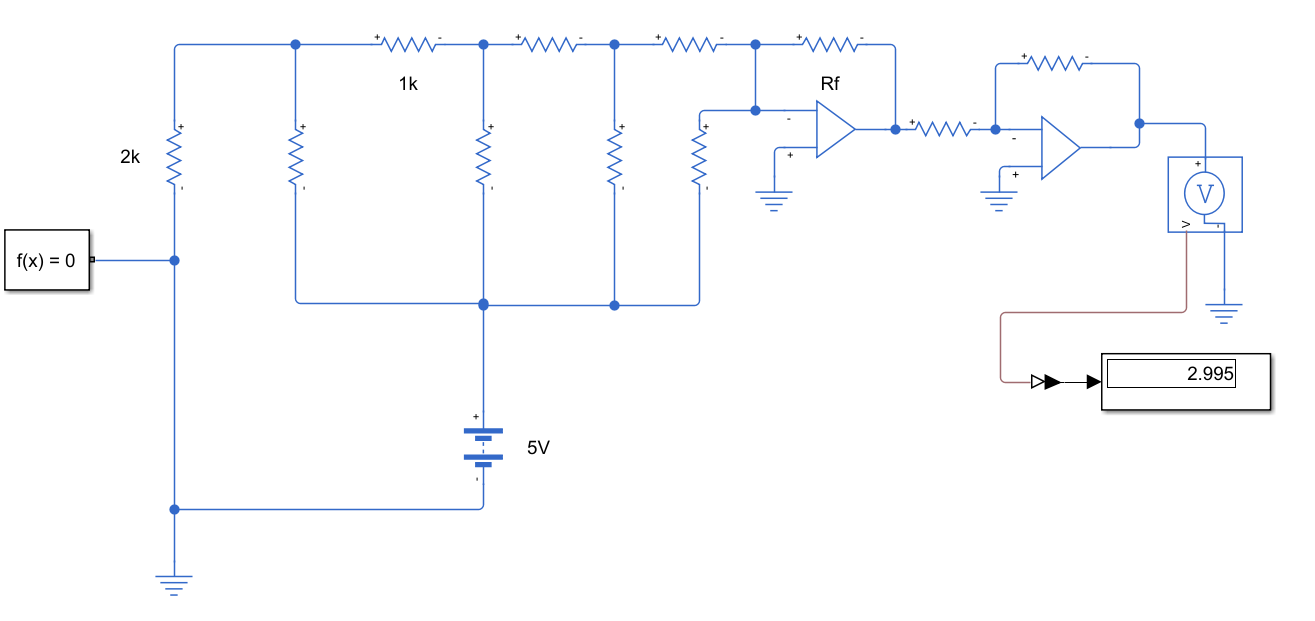
\includegraphics[width=0.75\linewidth]{Media/DAC2-iii.png}
\end{figure}

\section*{Question 3}
"a) Calculate the exact values of VL and VH  for this circuit.\\
b) Verify your solution using MATLAB\\
Note: The voltage supply is $V_{+}=5V$ and $V_{-}=0V$"

\noindent
a)\\
Finding $V_h$:\\
Assuming $V_{out} = 0V$, the comparator approaches the positive rail when $V_+ > V_- = 2$. and $V_+ = V_{in} - 100I$ where $I = \frac{V_+-V_{out}}{1k} = 2mA$.\\
So $V_{in}-0.2>2 \rightarrow V_{in} > 2.2V$, therefore $V_h = 2.2V$.

\noindent
Finding $V_l$:\\
Assuming $V_{out} = 5V$, the comparator approaches the negative rail when $V_+ < V_- = 2$. and $V_+ = V_{in} - 100I$ where $I = \frac{V_+-V_{out}}{1k} = -3mA$.\\
So $V_{in}+0.3>2 \rightarrow V_{in} < 1.7V$, therefore $V_l = 1.7V$.\\

\noindent
b) (I don't know how to turn the knob while the simulation is running)
\begin{figure}[h]
    \centering
    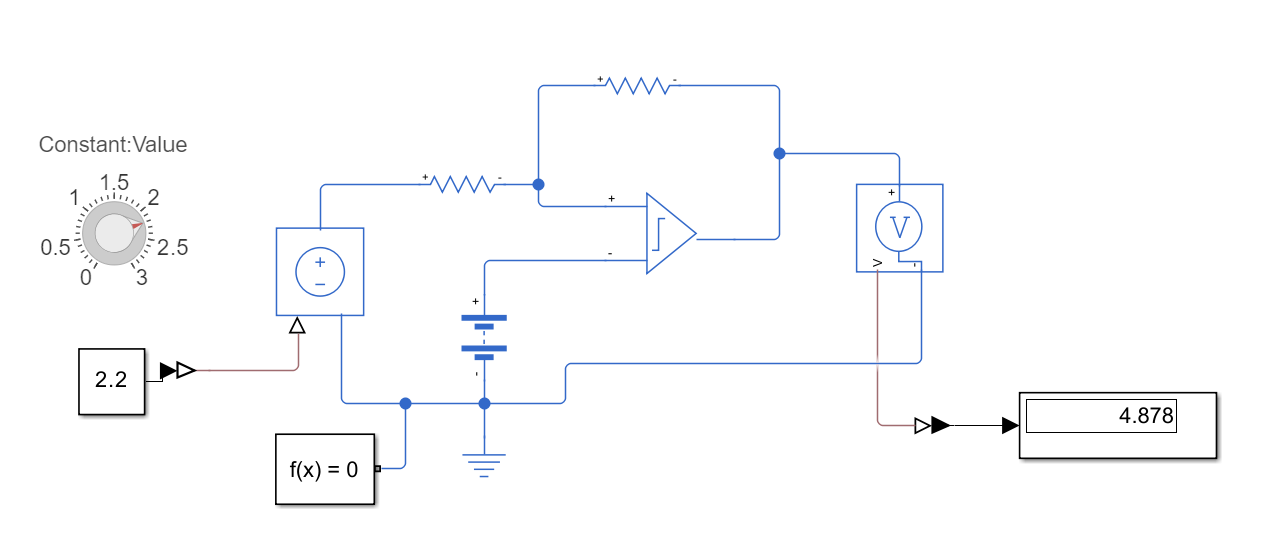
\includegraphics[width=0.75\linewidth]{Media/Vh.png}
\end{figure}

\begin{figure}[h]
    \centering
    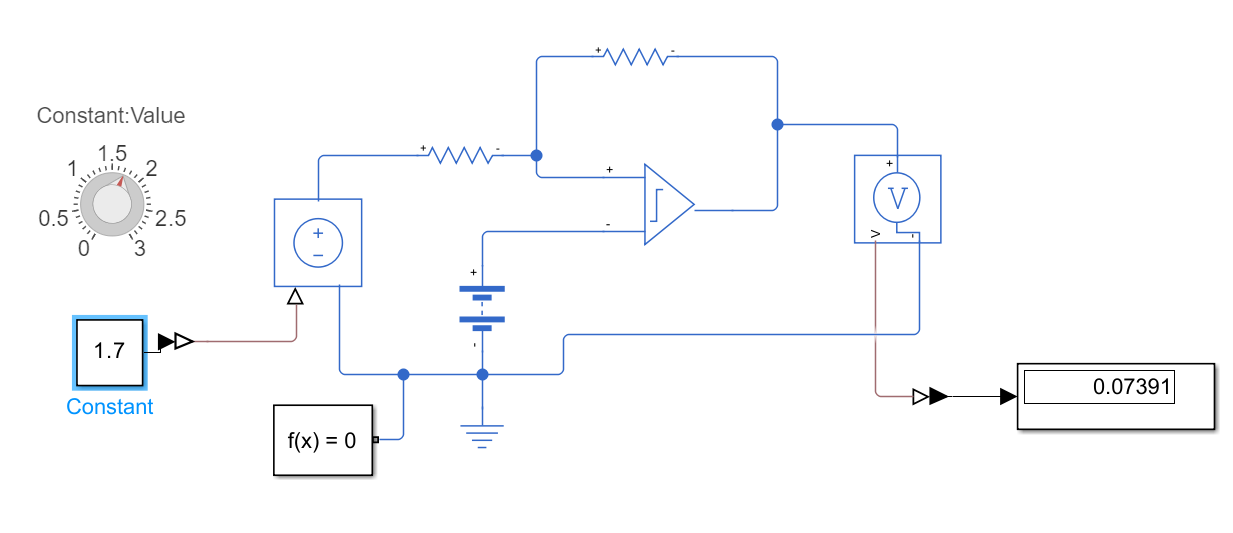
\includegraphics[width=0.75\linewidth]{Media/Vl.png}
\end{figure}

\end{document}
